\chapter{Appendix}

\section{Testfälle} \label{tests}

\begin{longtable}{|p{1cm} | p{10cm} |p{1.2cm} |}
  \hline
    ID & Ablauf & Erfüllt \\\hline
    T1 & Das (allgemeine) Kontextmenü öffnen und im Untermenü \textit{Add New} den entsprechenden Typ auswählen. Danach öffnet sich ein Dialog, wo der neue \gls{Node} beschrieben werden kann. Nach dem Speichern muss er an der Stelle, wo das Kontextmenü aufgerufen worden ist, angezeigt werden. & Ja \\\hline
    T2 & Das \gls{Node}-Kontextmenü öffnen und im Untermenü \textit{Link To} den entsprechenden Typ auswählen. Danach öffnet sich ein Dialog, wo der neue \gls{Node} beschrieben werden kann. Nach dem Speichern muss der Node, bei welchem das Kontextmenü aufgerufen wurde, mit einem Link zum neuen Node verbunden sein und in der Umgebung darstellt werden. & Ja \\\hline
    T3 & Das (allgemeine) Kontextmenü öffnen und im unteren Bereich den darzustellenden \gls{Node} suchen und auswählen. Danach muss er an der Stelle, wo das Kontextmenü aufgerufen worden ist, zusammen mit seinen Kind-\gls{Node}[s] und den verbindenden Links ersichtlich sein. & Ja\\\hline
    T4 & Das \gls{Node}-Kontextmenü öffnen und im Untermenü \textit{Link To} \textit{Existing Node} auswählen. Danach öffnet sich ein Dialog, wo der bestehende \gls{Node} gesucht und ausgewählt werden kann. Nach dem Speichern muss dieser mit dem Node, auf dem das Kontextmenü aufgerufen wurde, mit einem Link verbunden sein und in der Umgebung dargestellt werden. & Ja\\\hline
    T5 & Aus der Suche einen \gls{Node} per \gls{Drag'n'Drop}  in die Visualisierung ziehen und an einer freien Stelle loslassen. An dieser Stelle muss nun dieser \gls{Node} dargestellt werden. Für die mobile Ansicht muss zuerst die Suche über das entsprechende Icon geöffnet werden. Sobald der \gls{Drag'n'Drop} Prozess beginnt, verschwindet das Suchfeld, um den \gls{Node} optimal positionieren zu können, nach dem Loslassen wird es wieder dargestellt. & Ja \\\hline
    T6 & Aus der Suche einen \gls{Node} per \gls{Drag'n'Drop} in die Visualisierung ziehen und über einem bereits dargestellten \gls{Node} loslassen. Nun muss dieser \gls{Node} mit dem ausgewählten \gls{Node} per Link verbunden werden. Für die mobile Ansicht muss zuerst die Suche über das entsprechende Icon geöffnet werden. Sobald der \gls{Drag'n'Drop}-Prozess beginnt, verschwindet das Suchfeld, um den \gls{Node} optimal positionieren zu können, nach dem Loslassen wird es wieder dargestellt. & Ja \\\hline
    T7 & Das \gls{Node}-Kontextmenü öffnen und mit \textit{Hide Node} den entsprechenden \gls{Node} ausblenden. Dabei müssen alle ein- und ausgehenden Links ebenfalls ausgeblendet werden. & Ja\\\hline
    T8 & Das \gls{Node}-Kontextmenü öffnen und mit \textit{CollapseAllLinks} alle ausgehenden Links ausblenden. Falls der Ziel-\gls{Node} des jeweiligen \gls{Node}[s] keinen anderen ein- oder ausgehenden Link besitzt, muss dieser auch ausgeblendet werden. & Ja\\\hline
    T9 & Das \gls{Node}-Kontextmenü öffnen und mit \textit{ExpandAllLinks} alle ausgehenden Links einblenden. Falls der Ziel-\gls{Node} nicht bereits eingeblendet ist, muss dieser zusammen mit dem Link eingeblendet werden. & Ja\\\hline
    T10 & Das \gls{Node}-Kontextmenü öffnen und im unterem Bereich einen ausgehenden Link auswählen, dieser muss anschliessend zusammen mit dem Ziel \gls{Node}, falls dieser noch nicht dargestellt ist, dargestellt werden. & Ja\\\hline
    T11 & Die auszublendenden Links in der Visualisierung auswählen, diese werden pink gefärbt. Danach in der Toolbar mit \textit{COLLAPSE} ausblenden. & Ja \\\hline
    T12 & In der Navigation im Menu \textit{View}, \textit{New View} auswählen. Die Visualisierung wird aktualisiert mit einer leeren \gls{View}. & Ja\\\hline
    T13 & Eine neue \gls{View} erstellen einen beliebigen \gls{Node} darstellen, danach den Browser schliessen und neu öffnen. Nun muss die zuvor erstellte \gls{View} ebenfalls verfügbar und der eben erstelle \gls{Node} sollte sichtbar sein. & Ja\\\hline
    T14 & Titel eines \gls{Node}[s] in der Datenbasis aktualisieren. Dieser muss auch in der Visualisierung aktualisiert sein. & Ja\\\hline
    T15 & Einen \gls{Node} in der Datenbasis löschen. Dieser muss auch aus allen \gls{View} gelöscht sein. & Ja\\\hline
    T16 & Einen Link aus der Datenbasis löschen. Dieser darf nicht mehr in den \gls{View} dargestellt werden. &Ja\\\hline
    T17 & Einen Link in der Datenbasis erstellen. Dieser darf nicht dargestellt werden, muss aber bei dem entsprechenden \gls{Node} zur Auswahl stehen für die Darstellung. & Ja\\\hline
    T18 & Einen bestehenden \gls{Node} mit mehr als sieben ausgehenden \gls{Node}[s] darstellen. Es dürfen dabei nicht mehr als sieben Links dargestellt werden. & Ja\\\hline
    T19 & In der Toolbar mit \textit{SHOW LINK LABEL} bzw. \textit{HIDE LINK LABEL} die Labels der Links ein oder ausblenden. & Ja\\\hline
    \caption{Testfälle Beschreibung}
  \label{tab:testkonzept-detail}
\end{longtable}



\section{User-Stories}

\begin{longtable}{|p{1cm} | p{10.8cm} |}
\hline
ID  & Description\\ \hline
S1  & Die Schnittstellen und die Model-Klassen für die Implementierung definieren.     \\ \hline
S2  & Das Projektteam erhält einen Überblick über den aktuellen Stand der Technik. Es soll eine Auswahl von vier möglichen Frameworks getroffen werden.\\ \hline
S3  & Detail Beurteilung zweier Frameworks anhand des Standard-Szenarios.\\ \hline
S4  & Detail Beurteilung zweier Frameworks anhand des Standard-Szenarios. \\ \hline
S5  & Definition des Standard-Szenarios zur genaueren Beurteilung der vier möglichen Frameworks. \\ \hline
S6  & Mock-up aller Benutzeroberflächen erstellen \\ \hline
S7  & Anbindung des Interface-Paket (\textit{ikc-visual}) via NPM Setup. Typescript- und React-Setup des Projekts im Gitlab \\ \hline
S8  & Der Benutzer kann einen \gls{Node} z.B. aus der Suche von ausserhalb in die Visualisierung ziehen. Wird der \gls{Node} an einer freien Position losgelassen, wird dieser der Visualisierung an dieser Stelle hinzugefügt. Wird er jedoch über einem bestehenden \gls{Node} losgelassen, wird ein neuer Link zu diesem erstellt und der neue \gls{Node} in seiner Umgebung platziert. Dies soll sowohl im mobilen als auch auf im Desktop-Umfeld möglich sein. Der entsprechende \gls{Node} wird immer zusammen mit all seinen Kindern angezeigt. Sind es mehr als sieben, werden nur sieben angezeigt und der Rest über das Kontext-Menü zugänglich gemacht.\\ \hline
S9  & Einen \gls{Node} in der Visualisierung kann per \gls{Drag'n'Drop} positioniert werden. Diese Position muss gespeichert werden.    \\ \hline
S10 & Werden zwei \gls{Node}[s] in der Visualisierung aufeinander gezogen, sollen zwei beschriftete Links entstehen, jeweils in eine Richtung.       \\ \hline
S11 & Mittels eines Kontext-Menüd kann der Benutzer neue \gls{Node}[s] erstellen und die Visualisierung hinzufügen oder einen bestehenden hinzufügen. Dies geschieht an der Stelle, wo das Menü aufgerufen wurde. Das Menü öffnet sich durch einen Rechtsklick oder einen langen Tap. Das Suchfeld wird vom \gls{ikc-core} geliefert werden. \\ \hline
S12 & Der Benutzer kann durch einen Rechtklick auf einen \gls{Node} oder einen langen Tap das \gls{Node} Kontext-Menü aufrufen. Dort soll er die folgenden Möglichkeiten haben: \textit{Edit Node}, \textit{Hide Node} \textit{LinkToExistingNode}, \textit{LinkToNewNode} (Link zu einem bestehenden \gls{Node} erstellen oder einen neuen \gls{Node} erstellen und dann verlinken, der entsprechende \gls{Node} wird in der Umgebung angezeigt), \textit{CollapseAllLinks} (alle ausgehenden Links verstecken), \textit{ExpandAllLinks} (alle ausgehenden Links anzeigen) \textit{SearchLinks} (Versteckte Links druchsuchen und einzeln anzeigen können, die Suche soll sowohl den Titel des Ziel \gls{Node}[s] als auch das Label des Links verwenden) Das Suchfeld wird vom \gls{ikc-core} geliefert werden. \\ \hline
S13 & Links können separat ausgewählt und ausgeblendet werden.  \\ \hline
S14 & Die Labels der Visualisierung sollen versteckt oder angezeigt werden können.\\ \hline
S15 & Die Visualisierung soll in den bestehenden \gls{ikc-core} integriert werden. \\ \hline
S16 & Änderungen in der Visualisierung sollen in den \gls{ikc-core} als auch umgekehrt vom \gls{ikc-core} in die Visualisierung übernommen werden. \\ \hline
S17 & \gls{View}[s] sollen dauerhaft gespeichert werden. Ebenfalls sollen neue erstellt werden können.          \\ \hline
S18 & Es müssen die folgenden Dialoge bereitgestellt werden, \textit{SearchExistingNodeToConnect}, \textit{NewNodeToConnect} und \textit{NewNode}.\\ \hline
S19 & Es müssen zwei Suchfelder zur Verfügung gestellt werden: (\textit{NodeSearch} und \textit{LinkSearch})\\ \hline
    \caption{User Stories Beschreibung}
\label{user-stories-desc}
\end{longtable}

\section{Wichtigste Protokolle}
\label{protokolle}


\section{Arbeitsjournal}
\label{arbeitsjournal}


\section{Aufgabenstellung}
\label{aufgabenstellung}


\section{Anforderungsanalyse}\label{anforderungsanalyse-mk}

\includegraphics[page=1,scale=0.8]{kapitel/anforderungen.pdf}

\includegraphics[page=2,scale=0.8]{kapitel/anforderungen.pdf}

\includegraphics[page=3,scale=0.8]{kapitel/anforderungen.pdf}

\includegraphics[page=4,scale=0.8]{kapitel/anforderungen.pdf}

\section{Projektmanagement}

\newpage

\subsection{Projektstrukturplan}
\begin{landscape}
\begin{figure}[ht]
\centering
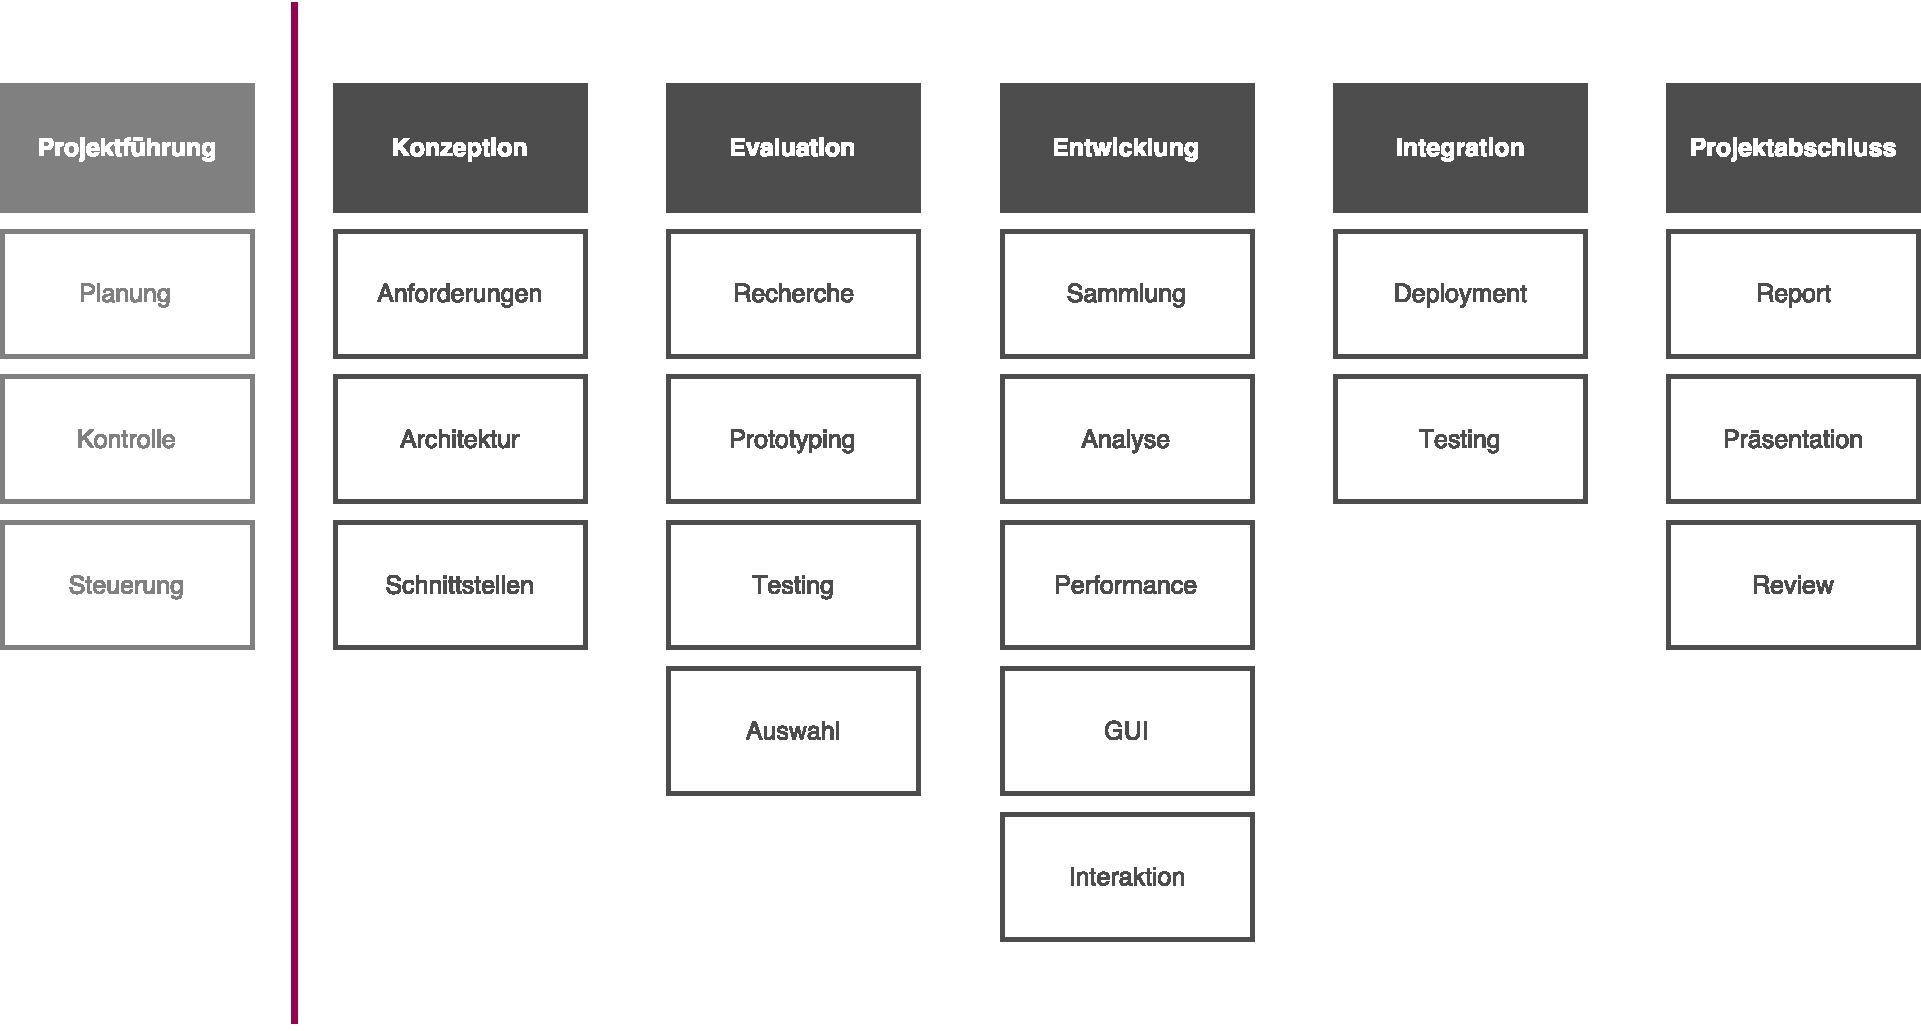
\includegraphics[width=1.5\textwidth]{Projektstrukturplan}
\caption{Projektstrukturplan}
\label{fig:projektstrukturplan}
\end{figure}
\end{landscape}

\newpage
\subsection{Meilensteine}

\begin{longtable}{|p{1cm}|p{2cm}|p{8.5cm}|}
  \hline
    ID & Datum &  Beschreibung \\\hline
    M1 & 19.09.2016 & Administrativer Meilenstein: Kickoff\\\hline
    M2 & 09.10.2016 & Administrativer Meilenstein: Projektplanung abgeschlossen\\\hline1
    M3 & 16.10.2016 & Entwicklung Meilenstein: Schnittstellen definiert\\\hline
    M4 & 06.11.2016 & Entwicklung Meilenstein: Evaluation Entscheid\\\hline
    M5 & 25.12.2016 & Entwicklung Meilenstein: Funktionsfähige Oberfläche umgesetzt\\\hline
    M6 & 15.01.2017 & Entwicklung Meilenstein: Integration in \gls{ikc-core} abgeschlossen\\\hline
    M7 & 22.01.2017 & Administrativer Meilenstein: 95\% erreicht\\\hline
    M8 & 30.01.2017 & Administrativer Meilenstein: PAWI Bericht Abgabe\\\hline
    M9 & 31.01.2017 & Administrativer Meilenstein: Präsentation\\\hline
    \caption{Meilensteine}
  \label{tab:meilensteine}
\end{longtable}
\subsection{Rahmenplanung}
\newpage

\begin{landscape}
\begin{figure}[ht]
\centering
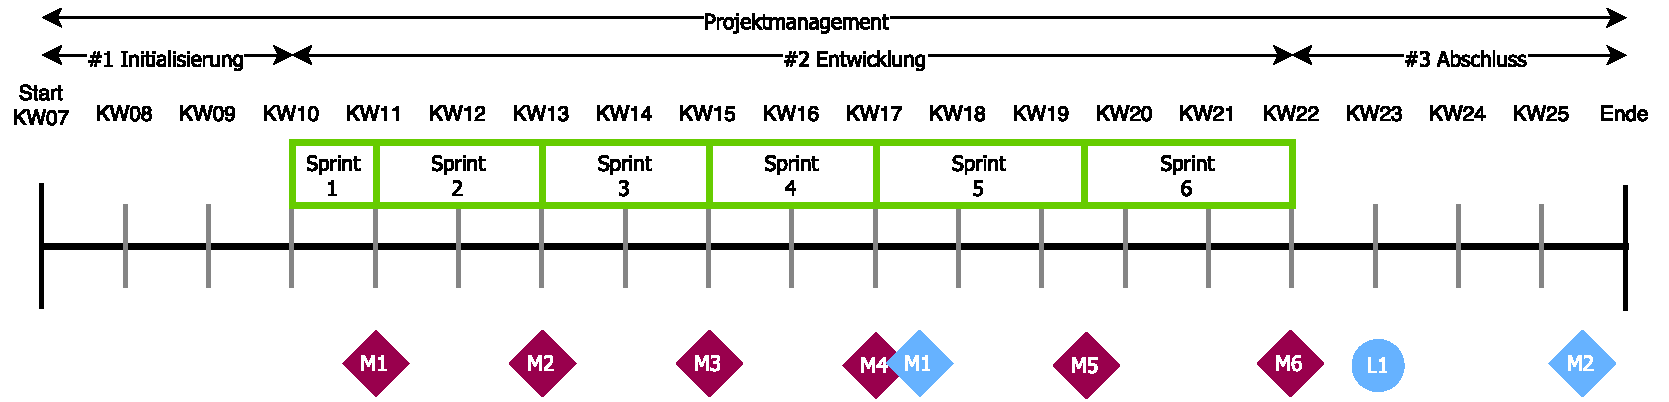
\includegraphics[width=1.7\textwidth]{Rahmenplan}
\caption{Rahmenplan}
\label{fig:rahmenplan}
\end{figure}
\end{landscape}

\newpage

\subsection{Anforderungen}
\begin{longtable}{|p{1.5cm} | p{1.5cm} | p{8.1cm}|}
  \hline
    ID & Priorität & Beschreibung \\\hline
    A1 & M & \gls{Datenquelle}[n] können mittels einer Autoindexierung automatisch in die Volltextsuche inventarisiert werden.\\\hline
    A2 & S & Neue oder geänderte Dateien können im bestehenden Index hinzugefügt oder geändert werden (z.B. automatisch nach Änderungs- oder Erstellunhgsdatum). Es ist zu prüfen, wie diese Änderung sich auf die bestehenden Tags auswirkt. \\\hline
    A3 & S  & Die zu indexierenden \gls{Datenquelle}[n] können vom Benutzer ausgewählt werden.\\\hline
    A4 & M & Mittels der Volltextsuche sollen sowohl alle Knoten, als auch alle in den \gls{Datenquelle}[n] enthaltenen Dokumente, welche in der Autoindexierung erfasst sind, durchsucht werden können.\\\hline
    A5 & M & Die Volltextsuche kann über ein Suchfeld genutzt werden.\\\hline
    A6 & C & Dabei sollen die unterschiedlichen Quellen der Resultate visuell unterschieden werden können.\\\hline
    A7 & M & Basierend auf dem Inhalt des Wissensnetzwerks sollen \gls{Keyword}[s] berechnet und dem User zur Verknüpfung vorgeschlagen werden.\\\hline
    A8 & M & Die automatisch generierten \gls{Keyword}[s] sind klar als solche gekennzeichnet und können vom Benutzer angenommen oder abgelehnt werden. (\gls{Tag Recommondation})\\\hline
    A9 & C & Mittels \gls{Tags} kann der Benutzer weitere Informationen zu Knoten hinzufügen.\\\hline
    A10 & C & Bestehende \gls{Tag}[s] sollen dem Benutzer vorgeschlagen werden.\\\hline
    A11 & M & Jedes Dokument, das der Benutzer in sein Netzwerk hinzufügt, wird als ein Knoten im Wissensnetzwerk eingefügt. Jeder \gls{Tag} eines solchen Dokuments wird auch als Knoten im Wissensnetzwerk eingefügt. Die zugehörigen Tags werden als  Links zwischen den Tag-Knoten und den Dokument-Knoten verbunden.\\\hline
    A12 & M & \gls{Tag}[s] werden dem User differenziert von den anderen Eigenschaften dargestellt.\\\hline
    A13 & C & Zusammengesetze Wörter (\gls{n-gram}[s]) werden als solche erkannt und entsprechend in der \gls{Keyword Extraction} berücksichtigt. \\\hline
    A14 & S & \gls{SFTP} Persistenz (DB), Index, Konfiguration \\\hline
    A15 & C & \gls{Dropbox} Persistenz (DB), Index, Konfiguration \\\hline
    A16 & C & \gls{Evernote} Index, Konfiguration \\\hline
    %A1 & M & Implementation einer Funktion \texttt{getRelevantTerms(Doc)}, welche pro Dokument eine sortierte Liste (nach tf-idf-Relevanz) von \gls{Keyword}[s] zurückgibt.\\\hline
    \caption{Funktionale Anforderungen}
  \label{tab:funktionale-anforderungen}
\end{longtable}

\begin{longtable}{|p{1.5cm} | p{1.5cm} | p{8.1cm}|}
  \hline
    ID & Priorität & Beschreibung \\\hline
    A1 & M & Die Autoindexierung soll den Benutzer nicht in der Bedienung blockieren (Usability).\\\hline
    A2 & M & Die \gls{Keyword Extraction} ist innerhalb nützlicher Frist abzulaufen. \\\hline
    A3 & S & Generische Einbindung der Quelle (zum Beispiel Factory-Pattern) für eine einfache Anbindung neuer Quellen.\\\hline
    A4 & M  & 360 Stunden pro Person\\\hline
    A5 & S & Arbeitsjournal \\\hline
    A6 & S & Weiterentwicklung des \gls{ikc-core}[s] \\\hline
    \caption{Nicht funktionale Anforderungen}
  \label{tab:nicht-funktionale-anforderungen}
\end{longtable}

\subsection{Risikoanalyse}\label{risikoanalyse}

In folgender \autoref{tab:risikoanalyse} werden mögliche Risiken behandelt. Die Wahrscheinlichkeit ist mit P abgekürzt. R steht für Risiko und S für den Schaden, welcher mittels $P*R=S$ berechnet wird. Die Skala reicht von eins bis fünf.

\clearpage

\begin{longtable}{|p{0.5cm} | p{7cm} | p{1cm}|  p{1cm}|  p{1cm}|}
  \hline
    ID & Beschreibung &  P & R & S \\\hline
    R1 & Die für eine reibungslose und intuitive Bedienung nötige Performance kann nicht gewährleistet werden.\newline\newline
    Javascript ist sowohl auf dem Client als auch auf dem Server lauffähig. Damit kann jeweils auf die für den Anwendungsfall nötige Plattform gewechselt werden. & 3 & 4 & 12\\\hline
    R2 & Die Abgrenzung vom laufenden Projekt \textbf{\acrshort{IKC}} (vgl. \autoref{sec:scope}) ist klar festzulegen und einzuhalten. So können Überschneidungen und Unklarheiten verhindert werden.\newline\newline
    Vollständige und detaillierte Arbeitsjournale, wie auch Protokolle bieten dabei eine wichtige Hilfestellung. & 2 & 1 & 2\\\hline
    R3 & Die Zahl und auch der Schwierigkeitsgrad der Anforderungen ist hoch. Die Arbeit ist mit insgesamt 720 Stunden in einem grösseren Rahmen. Es ist daher möglich, dass nicht alle Anforderungen erfüllt werden.\newline\newline Eine strikte Priorisierung und ein funktionierendes Projektmanagement garantiert, dass wichtige Anforderungen erkannt und gleichzeitig auch nicht aus den Augen verloren werden. & 3 & 1 & 3\\\hline
    R4 & Typescript (beziehungsweise Javascript) ist für den Einsatzzweck nicht vollends geeignet und schränkt die Performance und oder den Einsatz von bestimmten Bibliotheken ein.\newline\newline
    Das Resultat dieser Arbeit ist ein Prototyp. Das Ziel ist damit den Mehrwert aus dem zusätzlichen Wissen aufzuzeigen. Sollte die Performance mit den genutzten Technologien nicht ausreichend sein, können dennoch diverse Konzepte und Erkenntnisse in einem Folgeprojekte wiederverwendet und weiterentwickelt werden.& 3 & 3 & 9\\\hline
    R5 & Demo-Daten und nur englische Dokumente & 3 & 1 & 3\\\hline
    \caption{Risikoanalyse}
  \label{tab:risikoanalyse}
\end{longtable}

\subsection{Lieferobjekte}

\begin{longtable}{|p{1cm} | p{2cm} | p{8.1cm}|}
  \hline
    ID & Datum &  Beschreibung \\\hline
    L1 & 26.04.2017 & Zwischenpräsentation.\\\hline
    L2 & 09.06.2017 & Funktionsfähige Software mit folgenden Eigenschaften:
    \begin{itemize}
        \item ...
    \end{itemize}
    \\\hline
    L3 & 09.06.2017 & Dokumentierter Sourcecode (für Methoden und Parameter).\\\hline
    L4 & 09.06.2017 & \gls{BDA}-Bericht.\\\hline
    \caption{Vorgegebene Lieferobjekte}
  \label{tab:set-lieferobjekte}
\end{longtable}
 
\begin{longtable}{|p{1cm} | p{2cm} | p{8.1cm}|}
  \hline
    ID & Datum &  Beschreibung \\\hline
    L1' & 24.03.2017 & Abschluss der Anforderungsanalyse.\\\hline
    L2' & 31.03.2017 & Konzeptioneller Prototyp, welcher aufgrund der Resultate der Technologierecherche entwickelt wurde.\\\hline
    L3' & 14.04.2017 & Integration des Prototypen in den \gls{ikc-core}\\\hline
    L3' & 26.05.2017 & Abschluss der Programmierung.\\\hline
    \caption{Zusätzliche, interne Lieferobjekte}
  \label{tab:add-lieferobjekte}
\end{longtable}



\subsection{Stories}
Die User-Stories repräsentieren alle Arbeitspakete, welche über die gesamte Projektdauer geplant wurden. Diese werden nicht nur im klassischen Sinne für die Klassifizierung von Applikationsfunktionen, sondern auch für konzeptionelle Aufgaben verwendet. Insgesamt haben wurde der Aufwand mit \textbf{256} Punkte beziffert, wobei ein Punkt circa einer Stunde entspricht. Dies entspricht auch etwa dem resultierenden Aufwand von \textbf{276} Punkten. Der Mehraufwand konnte dank einiger Reserven gut kompensieren werden. Dieser entstand vor allem in der Umsetzung der \gls{Drag'n'Drop} Gesten und dem Datenaustausch zwischen \gls{ikc-core} und Visualisierung. Alle User-Stories sind in der \autoref{user-stories} detailliert aufgelistet und die weiterführenden Beschreibungen sind in der \autoref{user-stories-desc} zu finden.
\begin{longtable}{|p{0.6cm}|P{3.5cm}|p{1.4cm}|p{1.4cm}|p{2.4cm}|p{1.1cm}|}
\hline
ID  & Name & Geplant & Effektiv &Sprint\\ \hline
S1 & Technologierecherche           & 40 pt             &  pt              & 1, 2 \\ \hline
S1 & Definition Projektrahmen           & 40 pt             &  pt              & 1  \\ \hline
S1 & Entwurf Anforderungen           & 40 pt             &  pt              & 1 \\ \hline
S1 & Setup Dokumentation           & 40 pt             &  pt              & 1 \\ \hline
S1 & Prototype Keyword Extraktion            & 40 pt             &  pt              & 2 \\ \hline
S1 & Tokenauthentifizierung           & 40 pt             &  pt              & 2 \\ \hline
S1 & Keyword Extraktion grosser Index          & 40 pt             &  pt              & 2, 3 \\ \hline
S1 & Integration Suche in Index in Benutzeroberfläche           & 40 pt             &  pt              & 3 \\ \hline
S1 & Keyword Extraktion für bestimmtes Dokument         & 40 pt             &  pt              & 3 \\ \hline
S1 & Extraktion aller Dokumente für ein Keyword       & 40 pt             &  pt              & 3 \\ \hline
S1 & Optimierung Keyword Extraktion Algorithmus    & 40 pt             &  pt              & 3,4,6 \\ \hline
S1 & Begrenzung der extrahierten Keywords    & 40 pt             &  pt              & 3,4,6 \\ \hline
S1 & Begrenzung Dokumente für Keywords    & 40 pt             &  pt              & 3,4,6 \\ \hline
\hline
 & \textbf{Total}                       & \textbf{256 pt}             & \textbf{276 pt}               &  &  \\ \hline
    \caption{User Stories}
 \label{user-stories}
\end{longtable}

\subsection{Testkonzept}
Basierend auf den \hyperref[anforderungen]{Anforderungen} wurden die verschiedenen Testfälle definiert. Diese sind hier zusammengefasst. Konkret handelt es sich um die folgenden Testfälle (\autoref{tab:testkonzept}), welche im \autoref{tests} genauer beschrieben sind.

\begin{longtable}{|p{1cm} | P{6cm} |}
  \hline
    ID & Kurzbeschrieb \\\hline
    T1 & \gls{ikc-core} starten, Index existiert nicht.\\\hline
    T2 & \gls{ikc-core} starten, Index existiert ist jedoch nicht initialisiert.\\\hline
    T3 & \gls{ikc-core} starten, Index existiert und ist initialisiert.\\\hline
    T4 & Dokument suchen innerhalb des Index.\\\hline
    T5 & \gls{Keyword}[s] für ein Dokument abfragen.\\\hline
    T6 & Dokumente für \gls{Keyword} abfragen.\\\hline
    T7 & Neues Dokument erstellen.\\\hline
    T8 & Dokument ändern.\\\hline
    \caption{Testfälle}
  \label{tab:testkonzept}
\end{longtable}


\section{Experten-Workshop}

\subsection{Problemstellung BDA}



\subsection{BDA Kevin Stadelmann}

\subsubsection{Problemstellung}

\begin{enumerate}
    \item Big Data, verteilte Cloud-Services, verteilte Informationsquellen $\rightarrow$ einfache Verknüpfung erschwert
    \item Komplexes Wissensmanagement
    \item Zugriffsberechtigung
    \item Heterogene Arbeitskulter im Informationsmanagement
    \item Kollaboration
\end{enumerate}

\subsubsection{Lösung}

\begin{enumerate}
    \item Meta-Service
    \item Benutzerdefiniertes Tagging
    \item Zentrales Suchinterface (Filterung) $\rightarrow$ direkter Zugriff auf die Datenquelle auf der jeweilgen Plattform
    \item Intelligente Suche: Software lernt aus dem Suchverhalten eines Nutzers:
    \begin{enumerate}
        \item Automatische Priorisierung
        \item Automatische Hervorhebung
        \item Ähnliche, passende Dokumente vorschlagen
        \item Zuletzt geänderte Dokumente vorschlagen
    \end{enumerate}
    \item Vernetzung der Informationen zu einem Wissensnetzwerk
    \item Automatisierte Verknüpfung durch einen Algorithmus
\end{enumerate}

\subsection{Überblick Funktionalität}

\begin{itemize}
    \item Volltextsuche über alle Dokumente der angegebenen Quellen (Autoindexierung)
    \item Automatische Einbindung relevanter Begriffe eines Dokumentes (Extraktion relevanter Schlüsselwörter)
\end{itemize}

Wo werden die Funktionen erwartungshalber innerhalb des \gls{ikc-core}[s] eingebunden?

\subsection{Erwartungen der Experten}


\subsection{Demonstration}

Umsetzung, Funtionalität

\begin{itemize}
    \item Volltextsuche über verknüpfte Dokumente und Nodes im Wissensnetzwerk.
    \item Auto-Indexierung aller verknüpften Dokumente.
    \item Automatische Zusammenfassung von Dokumenten anhand wichtigster Wörter (Keyword-Extraction).
    \item Die gefundenen Wörter werden automatisch Teil des Wissensnetzwerks.
    \item Auffinden ähnlicher Dokumente mithilfe der automatisch ermittelten wichtigsten Wörter im Wissensnetzwerk.
    \item Benutzerdefiniertes und automatisches Tagging.
\end{itemize}

\subsection{Fragen \& Diskussion}

Allgemein

\begin{itemize}
    \item Potential
    \item Mehrwert
    \item Chancen
    \item Gefahren
    \item Risiken
\end{itemize}


\begin{itemize}
    \item Welche Probleme könnten durch die Erweiterungen abgedeckt werden?
    \item Wo gibt es Verbesserungsmöglichkeiten?
    \item Allfällige Unklarheiten?
    \item Möglicher Einsatz in der Praxis?
    \item Kundenbezogen: B2B, B2C, Handelsbeziehung
\end{itemize}